
\section{Betriebsszenarien}
\label{s:Betriebsszenarien}
Betriebsszenarien helfen die vorher beschriebenen Betriebs- und Infrastrukturkosten in Anwendung zu bringen 
und eine mögliche Entwicklung in der nahen Zukunft aufzuzeigen. 
Die Größe des Flughafens beeinflusst die Infrastrukturkosten. 
Bei einem größeren Flughafen werden die Betriebsdifferenzen deutlicher, da das Verkehrsaufkommen wesentlich höher ist.
Größere Flughäfen fertigen täglich mehr Flugzeuge als Regionalflughäfen ab, 
was dazu führt, dass mehr Abfertigungsplätze umgerüstet und versorgt werden müssen,
wodurch mehr Arbeitskräfte geschult werden müssen.

Deshalb wird für die Betriebsszenarien der Flughafen Frankfurt gewählt,
welcher als bedeutendes Luftverkehrsdrehkreuz fungiert
und zudem der größte Verkehrsflughafen Deutschlands ist.
Der Fraport meldete im Jahr 2023 insgesamt 423764 gewerbliche Flugbewegungen, was im Durchschnitt 1160 Flugbewegungen pro Tag ausmacht. 
Es wird angenommen, dass die Hälfte davon Abflüge sind, also müssen 580 Flugzeuge pro Tag abgefertigt werden.
%
Die Gesamtbewegungen teilen sich nach Entfernungen folgend auf \cite{fraport2023frankfurt}:
\begin{itemize}
    \item Kurzstrecken (bis 2500 km) sind bei 72,8 \%;
    \item Mittelstrecken (bis 6000 km) sind 9,3 \%;
    \item Langstrecken (ab 6000 km) die restlichen 17,9 \%. 
    \end{itemize}
Da nicht explizit definiert wird, welche Entfernungen die Flugzeuge zurücklegen, werden die Betriebskosten anhand vorher beschriebener Distanzen berechnet.
Dabei wird für Kurzstrecken eine Entfernung von 400 km und für Langstrecken eine Distanz von 6000 km angenommen.
Für Mittelstrecken werden die selben Werte wie bei Langstreckenflügen verwendet, jedoch mit einer anderen Distanz von 4000 Kilometer,
dass Treibstoffverbrauch pro Stunde sich nicht ändern wird.

Anhand der zugrundeliegenden Informationen wird eine Flotte mit 580 Flugzeugen aufgestellt, in welcher alternative Antriebe eingesetzt werden.
Aufgrund der Flugeinschränkungen in der Nacht wird angenommen, dass die Flüge von 6 bis 24 Uhr gleichmäßig stattfinden. 
Wie bereits diskutiert wurde, können Kurzstrecken-Flüge durch den Einsatz von batteriebetriebenen Flugzeugen ersetzt werden, 
wobei hier als Ersatz auf SAF zurückgegriffen wird. Es ist nennenswert, dass nur ein Teil der tatsächlichen Nachfrage des Kurzstrecken-Bedarfs 
dadurch gedeckt werden kann. Die Mittel- und Langstrecken werden von Flugzeugen mit Wasserstoffturbine und SAF durchgeführt.
%
Durch Betrachtung des tatsächlichen Flugplans sind die Spitzenstunden eines Tages zu ermitteln, bei welchen Verkehrsfluss stärker als im Durschschnitt ist.
In diesem Fall werden höhere Infrastruktur- und Betriebskosten erwarten zu sein.
Um die Interpretation zu erleichtern, wird in dieser Arbeit angenommen, dass stündlich die gleiche Anzahl an Flugzeugen 
am Flughafen abgewickelt werden. 
%
Die Aufteilung der Antriebe für jedes Szenario ist in der Abbildung \ref{betriebsszenarien} dargestellt.
%
\begin{figure}[h]
	\centering
	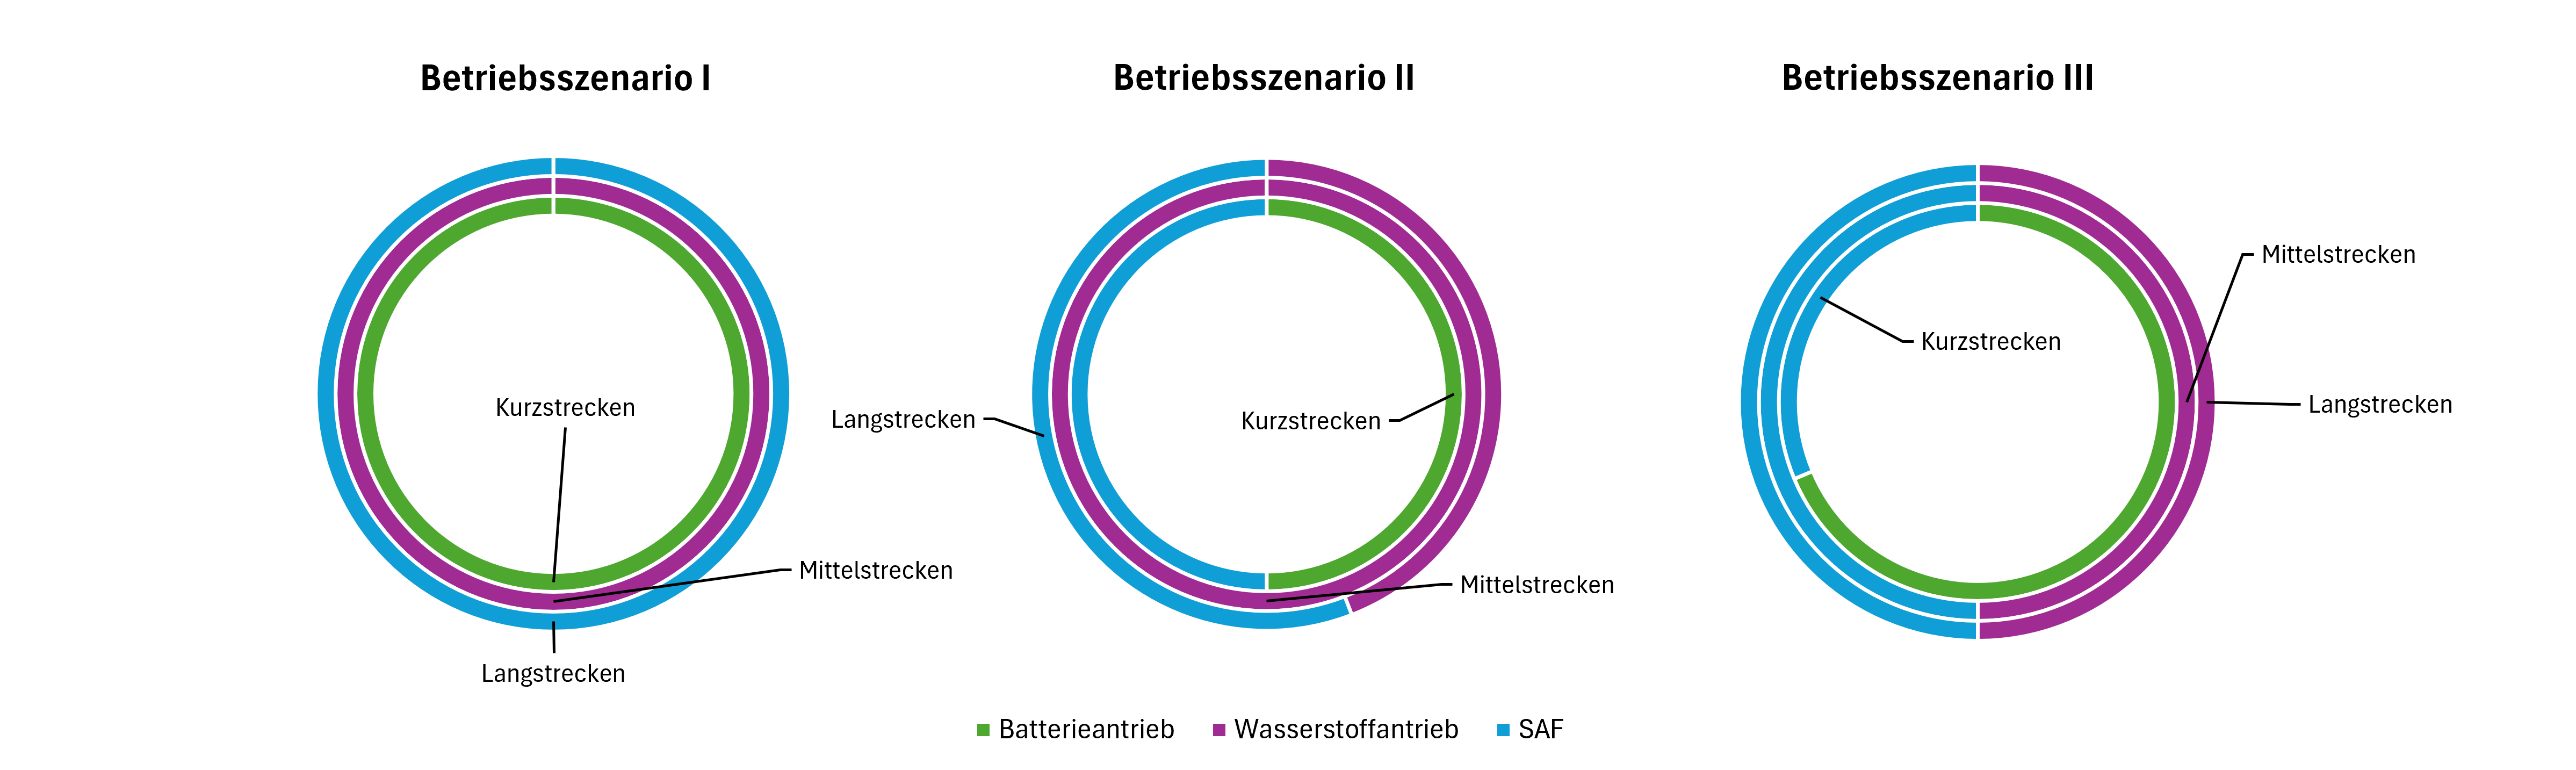
\includegraphics[width=1.0\linewidth]{Bilder/Betriebsszenarien.png}
	\caption[Betriebsszenarien]{Aufteilung der Flugzeugflotte nach Antriebsart}
	\label{betriebsszenarien}
\end{figure}
%
In dem \textbf{ersten Betriebsszenario} wird angenommen, dass:
\begin{itemize}
    \item Die Kurzstrecken durch den BA komplett ersetzt werden;
    \item Die Mittelstrecken werden vollkommen durch WA und
    \item die Langstrecken durch SAF bedient.
\end{itemize}
Das \textbf{zweite Betriebsszenario} wird mit folgender Aufteilung berechnet:
\begin{itemize}
    \item 50 \% der Kurzstrecken wird durch BA und 50 \% durch SAF betrieben; 
    \item die Mittelstrecken werden, genau wie im ersten Szenario, komplett durch Wasserstoffflugzeuge betrieben und 
    \item Langstrecken werden zu 10 \% der Gesamtflotte durch SAF und der Rest durch Wasserstoff bedient.
\end{itemize}
Das \textbf{dritte Szenario}:
\begin{itemize}
    \item 50 \% der Kurzstrecken werden durch BA, die restlichen 22,8 \% mit SAF betrieben
    \item Mittelstrecken: 50 \% der Mittelstrecken werden mit WA und 50 \% mit SAF betrieben
    \item Langstrecken: 50 \% der Langstrecken werden mit WA und die 50 \% mit SAF betrieben
\end{itemize}
%
Daraus ergibt sich die folgende Flottenaufteilung für die einzelnen Szenarien:
\begin{table}[h]
	\begin{center}
    \caption{Werte und Annahmen der BA-Infrastruktur}
	\label{BA_Infrastrukturtab}
	\begin{tabular}{|c|c|c|>{\centering\arraybackslash}p{3cm}|c|}
		\hline
		\multicolumn{4}{|c|}{\textbf{Szenario I}} \\ \hline
		 & \textbf{Batterieantrieb} & \textbf{Wasserstoffantrieb} & \textbf{SAF} \\ \hline
		Kurzstrecken & 422 & - &-\\ \hline
      	Mittelstrecken & -  & 54 &- \\ \hline
		Langstrecken & - & - &104 \\ \hline
		\multicolumn{4}{|c|}{\textbf{Szenario II}} \\ \hline
		Kurzstrecken & 211 &- &211\\ \hline
      	Mittelstrecken &  - & 54 &- \\ \hline
		Langstrecken &- & 46  &58 \\ \hline
		\multicolumn{4}{|c|}{\textbf{Szenario III}} \\ \hline
		Kurzstrecken & 290 &- &132\\ \hline
      	Mittelstrecken &  - & 27 & 27 \\ \hline
		Langstrecken &  -& 52 &52 \\ \hline
	\end{tabular}
    \end{center}
\end{table}
